\documentclass[tikz,border=8pt]{standalone}
% Shared preamble for the paper's TikZ schematics (2026-09-07). \input this after \documentclass.
% Palette mirrors src/utils/paper_style.py (read = green, write = blue, map = teal, grey = controls).
\usepackage[T1]{fontenc}
\usepackage{inter}
\renewcommand{\familydefault}{\sfdefault}
\usepackage{amsmath,amssymb}
\usetikzlibrary{arrows.meta,calc,decorations.pathreplacing,positioning,backgrounds}

\definecolor{readc}{RGB}{27,127,107}
\definecolor{writec}{RGB}{47,85,201}
\definecolor{mapc}{RGB}{31,108,128}
\definecolor{accentc}{RGB}{184,134,11}
\definecolor{blk}{RGB}{232,232,232}
\definecolor{blkb}{RGB}{160,160,160}
\definecolor{txt}{RGB}{60,60,60}
\definecolor{note}{RGB}{110,110,110}
\definecolor{panel}{RGB}{245,245,245}

\tikzset{
  blk/.style={draw=blkb,fill=blk,rounded corners=1.2pt,minimum width=0.50cm,minimum height=0.28cm,inner sep=0pt,line width=0.4pt},
  up/.style={-{Stealth[length=1.3mm,width=1.1mm]},blkb,line width=0.45pt},
  dots/.style={blkb,line width=0.45pt,dotted},
  lab/.style={font=\small,text=txt},
  small/.style={font=\scriptsize,text=note},
  tok/.style={font=\ttfamily\small,text=txt,rotate=90,anchor=east},
  marker/.style={circle,inner sep=0pt,minimum size=0.36cm,text=white,font=\bfseries\scriptsize},
  attn/.style={-{Stealth[length=1.6mm,width=1.4mm]},line width=0.7pt},
  halo/.style={white,line width=2.4pt},
  flow/.style={-{Stealth[length=1.6mm,width=1.4mm]},line width=0.8pt},
  vec/.style={-{Stealth[length=1.8mm,width=1.5mm]},line width=0.9pt},
  thinvec/.style={-{Stealth[length=1.3mm,width=1.1mm]},line width=0.55pt},
  ptitle/.style={font=\small\bfseries,text=txt,anchor=north west,align=left},
}

% \vstack{name}{x}{y}{base colour}{shade list (4 entries, % of base)} — residual-stream cell in the LM grid
\newcommand{\vstack}[5]{%
  \begin{scope}[shift={(#2,#3)}]
    \foreach \s [count=\k] in {#5}{%
      \fill[#4!\s!white,draw=white,line width=0.3pt] (-0.15,{0.46-0.23*\k}) rectangle (0.15,{0.46-0.23*(\k-1)});
    }
    \draw[#4!60!black,line width=0.35pt,rounded corners=0.6pt] (-0.15,-0.46) rectangle (0.15,0.46);
    \coordinate (#1) at (0,0);
    \coordinate (#1-n) at (0,0.46);
    \coordinate (#1-s) at (0,-0.46);
    \coordinate (#1-e) at (0.15,0);
    \coordinate (#1-w) at (-0.15,0);
  \end{scope}}

% \bstack{name}{x}{y}{base colour}{shade list (5 entries)} — free-standing feature vector
\newcommand{\bstack}[5]{%
  \begin{scope}[shift={(#2,#3)}]
    \foreach \s [count=\k] in {#5}{%
      \fill[#4!\s!white,draw=white,line width=0.4pt] (-0.19,{0.7-0.28*\k}) rectangle (0.19,{0.7-0.28*(\k-1)});
    }
    \draw[#4!60!black,line width=0.4pt,rounded corners=0.8pt] (-0.19,-0.7) rectangle (0.19,0.7);
    \coordinate (#1) at (0,0);
    \coordinate (#1-n) at (0,0.7);
    \coordinate (#1-s) at (0,-0.7);
    \coordinate (#1-e) at (0.19,0);
    \coordinate (#1-w) at (-0.19,0);
  \end{scope}}

\begin{document}
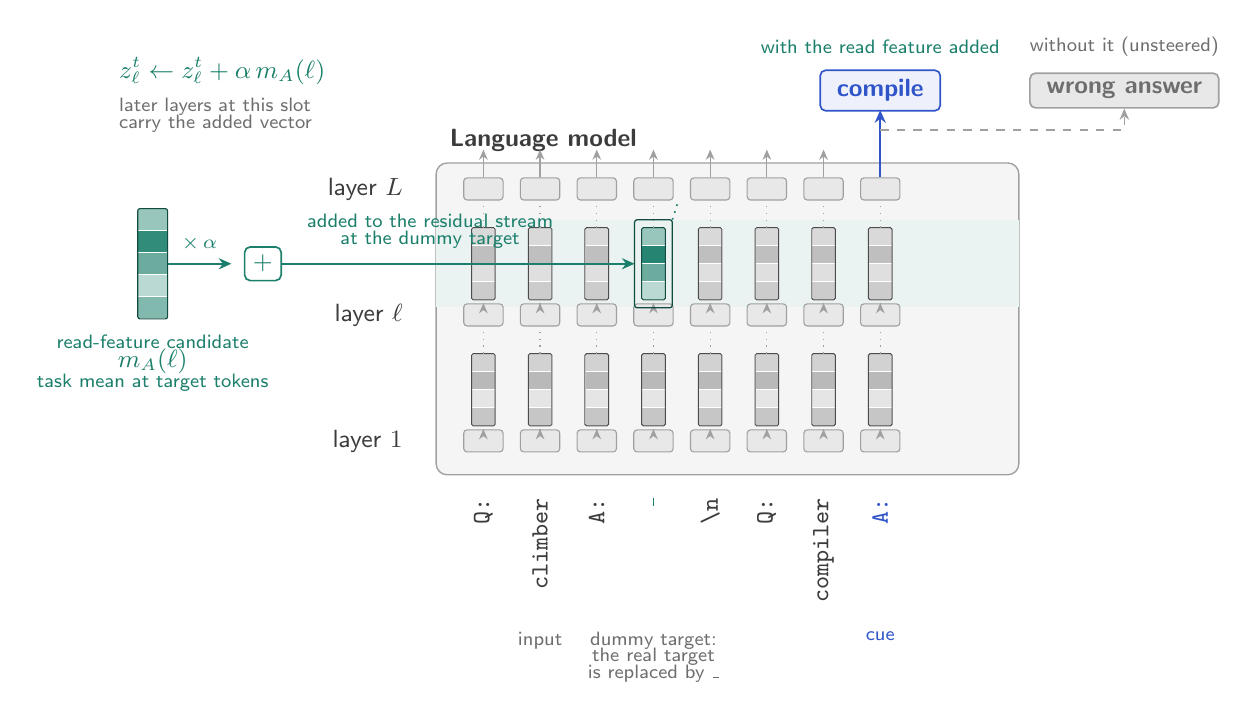
\begin{tikzpicture}[x=1cm,y=1cm]
% ---- geometry (same grid idiom as the circuit figure) ----
\def\dx{0.72}\def\xo{0.85}
\def\yLone{0.55}\def\yRone{1.20}\def\yLr{2.15}\def\yRr{2.80}\def\yLL{3.75}\def\yTop{4.25}
\begin{scope}[on background layer]
  \fill[panel,draw=blkb,rounded corners=4pt,line width=0.5pt] (0.25,0.12) rectangle (7.65,4.08);
  \fill[readc!9!white] (0.25,\yRr-0.55) rectangle (7.65,\yRr+0.55);
\end{scope}
\node[lab,font=\small\bfseries,anchor=south west] at (0.3,4.10) {Language model};

\foreach \tk/\role [count=\i] in {Q:/o, climber/i, A:/o, {\_}/d, {\char`\\n}/o, Q:/o, compiler/i, A:/c}{
  \pgfmathsetmacro{\x}{\xo+\dx*(\i-1)}
  \coordinate (c\i) at (\x,0);
  \node[blk] (b1-\i) at (\x,\yLone) {};
  \draw[up] (b1-\i.north) -- (\x,\yRone-0.5);
  \vstack{r1-\i}{\x}{\yRone}{gray}{35,55,20,45}
  \draw[dots] (r1-\i-n) -- (\x,\yLr-0.16);
  \node[blk] (br-\i) at (\x,\yLr) {};
  \draw[up] (br-\i.north) -- (\x,\yRr-0.5);
  \if\role d
    \vstack{rr-\i}{\x}{\yRr}{readc}{45,95,65,30}
  \else
    \vstack{rr-\i}{\x}{\yRr}{gray}{30,50,25,40}
  \fi
  \draw[dots] (rr-\i-n) -- (\x,\yLL-0.16);
  \node[blk] (bL-\i) at (\x,\yLL) {};
  \if\role c\else \draw[up] (bL-\i.north) -- (\x,\yTop); \fi
  \if\role d \node[tok,text=readc,font=\ttfamily\small\bfseries] at (\x,-0.05) {\tk};
  \else\if\role c \node[tok,text=writec,font=\ttfamily\small\bfseries] at (\x,-0.05) {\tk};
  \else \node[tok] at (\x,-0.05) {\tk};
  \fi\fi
}
% left labels
\node[lab,anchor=east] at (-0.05,\yLone) {layer $1$};
\node[lab,anchor=east] at (-0.05,\yLr) {layer $\ell$};

\node[lab,anchor=east] at (-0.05,\yLL) {layer $L$};
% token-role notes
\node[small,anchor=north,align=center] at ($(c4)+(0,-1.75)$) {dummy target:\\[-2pt]the real target\\[-2pt]is replaced by \texttt{\_}};
\node[small,anchor=north,align=center,text=writec] at ($(c8)+(0,-1.75)$) {cue};
\node[small,anchor=north,align=center] at ($(c2)+(0,-1.75)$) {input};

% ---- injection ----
\bstack{mA}{-3.35}{\yRr}{readc}{45,90,65,30,55}
\node[small,align=center,text=readc,anchor=north] at (-3.35,\yRr-0.78) {read-feature candidate\\[-1pt]{\small $m_A(\ell)$}\\[-1pt]task mean at target tokens};
\draw[flow,readc] (mA-e) -- (-2.35,\yRr) node[midway,above=1pt,small,text=readc] {$\times\,\alpha$};
\node[draw=readc,fill=white,rounded corners=2pt,line width=0.6pt,font=\small,text=readc,inner sep=3pt] (plus) at (-1.95,\yRr) {$+$};
\draw[flow,readc] (plus.east) -- ($(rr-4)+(-0.24,0)$)
  node[pos=0.42,above=2pt,small,text=readc,align=center] {added to the residual stream\\[-2pt]at the dummy target};
\draw[readc!60!black,line width=0.45pt,rounded corners=1pt] ($(rr-4)+(-0.24,-0.56)$) rectangle ($(rr-4)+(0.24,0.56)$);
% every later layer at this slot carries it
\draw[readc,line width=0.6pt,dotted] ($(rr-4)+(0.24,0.56)$) -- ($(bL-4.south east)+(0.06,0)$);

\node[small,text=readc,anchor=south west] at (-3.9,4.95) {\small $z^{t}_{\ell}\leftarrow z^{t}_{\ell}+\alpha\,m_A(\ell)$};
\node[small,anchor=south west,align=left] at (-3.9,4.35) {later layers at this slot\\[-2pt]carry the added vector};
% ---- outcome ----
\draw[flow,writec] (bL-8.north) -- ($(c8)+(0,4.75)$);
\node[draw=writec,fill=writec!8!white,rounded corners=2pt,line width=0.6pt,font=\small\bfseries,text=writec,minimum height=0.44cm,inner xsep=6pt] (good) at ($(c8)+(0,5.0)$) {compile};
\node[small,anchor=south,align=center,text=readc] at ($(good.north)+(0,0.08)$) {with the read feature added};

\node[draw=blkb,fill=blk,rounded corners=2pt,line width=0.6pt,font=\small\bfseries,text=note,minimum height=0.44cm,inner xsep=6pt] (bad) at ($(c8)+(3.1,5.0)$) {wrong answer};
\node[small,anchor=south,align=center] at ($(bad.north)+(0,0.08)$) {without it (unsteered)};

\draw[-{Stealth[length=1.4mm,width=1.2mm]},blkb,line width=0.6pt,dashed] ($(c8)+(0,4.5)$) -| (bad.south);
\end{tikzpicture}
\end{document}
